\documentclass{beamer}

\setbeamertemplate{navigation symbols}{}

\usepackage{graphicx}
\usepackage{amsmath, amssymb, amsfonts, amsthm}
\usepackage{tabularx}

\usetheme{CambridgeUS}


%-----------------------------------------------------------------------------------------------------------------
% New Environment for a plain box
\newenvironment{boxeded}
    {\begin{center}
    \begin{tabular}{|p{0.9\textwidth}|}
    \hline\\
    }
    { 
    \\\\\hline
    \end{tabular} 
    \end{center}
    }
%-----------------------------------------------------------------------------------------------------------------

% Die Präsentation dient dem Praxisprojekt: COVID-19 und wurde von Regina Galambos und Lorenz Mihatsch erstellt.

% Folgende Inhalte sollen besprochen werden: 
% 1: Datenstruktur und -erhebung erläutern:
% 1.1) Probleme der Erhebung: Recoding policy, testing policy.
% 2: Fallzahlen Weltweit als Timescale und als Weltkarte bezogen auf 100k Einwohner
% 3: Wachstumsraten der Fallzahlen
% 4: Ländervergleich. Zentrieren um Tag der Abriegelung irgendeiner Art.






%-----------------------------------------------------------------------------------------------------------------
% Presentation information: title, author.....

\title[Praxisprojekt: COVID-19]{Analyse der COVID-19 Fallzahlen}
\subtitle{Praxisprojekt}
\date{08. Mai 2020}
\author[R.Galambos, L.Mihatsch]{Regina Galambos, Lorenz Mihatsch\\
	
\includegraphics[width=0.22\textwidth]{LMU.pdf}\\
	{\small Projektpartner: Andr\'{e} Klima}\\
	{\small 08. Mai 2020}}

%-----------------------------------------------------------------------------------------------------------------


%-----------------------------------------------------------------------------------------------------------------
% Begin of presentation.

%Title page
\begin{document}
\begin{frame}
	\titlepage
\end{frame}

% Table of contents
\begin{frame}
   \frametitle{Inhaltsangabe}
   \tableofcontents
 \end{frame}
 
 
 % Einführung
 %-----------------------------------------------------------------------------------------------------------------
 \section{Einführung und Fragestellung}
 \begin{frame}
 	\frametitle{COVID-19 Pandemie}
 	\begin{enumerate}
 		\item COVID-19 ist ein Erkrankung, die durch das SARS-CoV-2 Virus ausgelöst wird.
 		\item Die Erkrankung ist erstmalig im Dezember 2019 in Wuhan (China) aufgetreten, der genaue Ursprung des Virus ist jedoch noch immer unbekannt.
 		\item Erster Erkrankungsfall in Deutschland am 28. Januar in Stockdorf.
 		\item Am 11. März wurde die ursprüngliche Epidemie (\emph{Def.} örtlich begrenztes Auftreten einer ansteckenden Krankheit) von der WHO als Pandemie (\emph{Def.} nicht mehr örtlich begrenztes Auftreten) eingestuft.
 		\item Am 22. März einigten sich Bund und Länder auf eine umfassende Beschränkung sozialer Kontakte.
 		\pause
 		\item \textbf{Wie haben sich die Zahl der Fälle und Todesfälle entwickelt?}
 	\end{enumerate}
 \end{frame}
 \section{Daten}
  
 \begin{frame}
 	\frametitle{Datengrundlage}
 	\begin{enumerate}
 		\item Anzahl an Fällen, Todesfällen und Genesenen
 		\begin{itemize}
 			\item Datensatz des \emph{Centers of Systems Science and Engineering} der Johns Hopkins University
 			\item Zusammentragung von Daten aus verschiedenen Quellen zu 213 Ländern. Bspw. \emph{Italy Ministry of Health}.
 			\item Täglich von \emph{RamiKrispin} auf GitHub aktualisiert und zu Verfügung gestellt. \url{https://github.com/RamiKrispin/coronavirus}
 	\pause
 		\end{itemize}
 		\item Demographie: Kontinentzugehörigkeit und Populationsdaten von 2018
 		\begin{itemize}
 			\item Datenbank der Weltbank und der UN. Zugriff über das R-package \emph{wbstat} und \emph{JohnSnowLabs} über \url{https://datahub.io/JohnSnowLabs/country-and-continent-codes-list}.
 		\end{itemize}
 	\pause
 		\item Politische Maßnahmen zur Eindämmung der Infektionsübertragung
 		\begin{itemize}
 			\item \emph{Government Response Tracker} Datesatz der \emph{University of Oxford}.
 			\item Zusammentragung von Daten zu politische Maßnahmen der einzelnen Länder aus verschiedenen Quellen.
 			\item \url{https://www.bsg.ox.ac.uk/research/research-projects/coronavirus-government-response-tracker}
 		\end{itemize}
 	\end{enumerate} 
 \end{frame}

 \begin{frame}
 	\frametitle{Anmerkungen zu den Daten}
 	\begin{enumerate}
 		\item Es handelt sich ``nur'' um die aufgezeichneten Fälle und Todefälle. (max. untere Schranke)
 		\item Starke Unterschiede in der Aufzeichnungs- und Testpolitik einzelner Länder, was einen direkten Ländervergleich schwer möglich macht. 
 		\item Die Kreuzfahrtschiffe Diamond Princess, Grand Princess und MS Zaandam wurden ausgeschlossen, da keinem Land eindeutig zuortbar. 
 		\item Die Zahl der Fälle und Todesfälle beziehen sich meist auf 100.000 Personen.
 		\item Analyse endet am 27. April 2020.
 		\pause
 		\item Programmierung einer Web-Application: \url{https://covid-19-stats-project.herokuapp.com}
 		\item Abbildungen sind auf Englisch da sie sich an ein ggf. internationales Publikum richten.
 	\end{enumerate}
 \end{frame}
 
 \section{Kumulativen Anzahl an Fällen und Todesfällen weltweit}
 \begin{frame}
 	\frametitle{COVID-19 weltweit}
	\begin{figure}
		\centering
		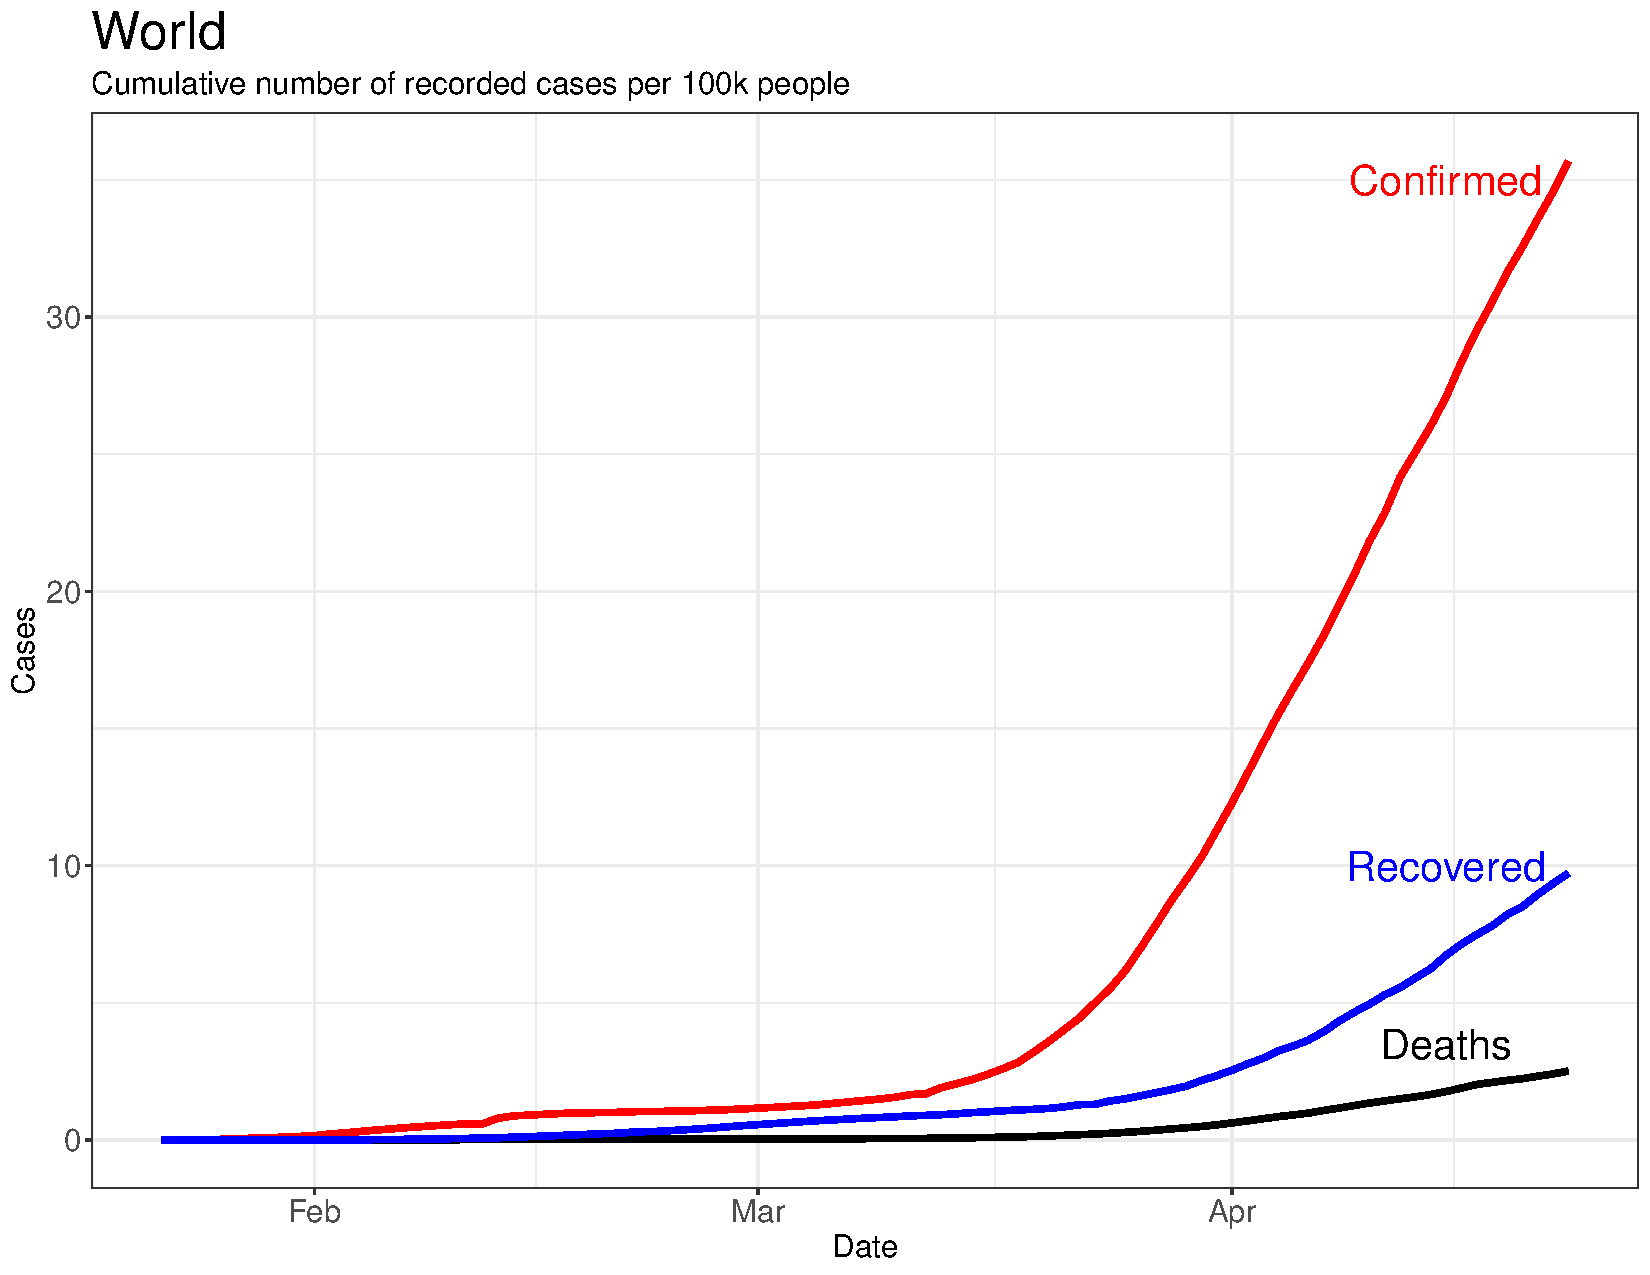
\includegraphics[width = 270pt]{Cases_world.pdf}
	\end{figure}
 \end{frame}

 \begin{frame}
 	\frametitle{COVID-19 weltweit}
		\centering
		\includegraphics[width = 350pt]{world_confirmed_mod.pdf}
 \end{frame}

 \begin{frame}
 	\frametitle{COVID-19 weltweit}
		\centering
		\includegraphics[width = 350pt]{world_death_mod}
 \end{frame}
 
 \begin{frame}
 	\frametitle{COVID-19 weltweit bestätigte Fälle}
	\begin{figure}
		\centering
		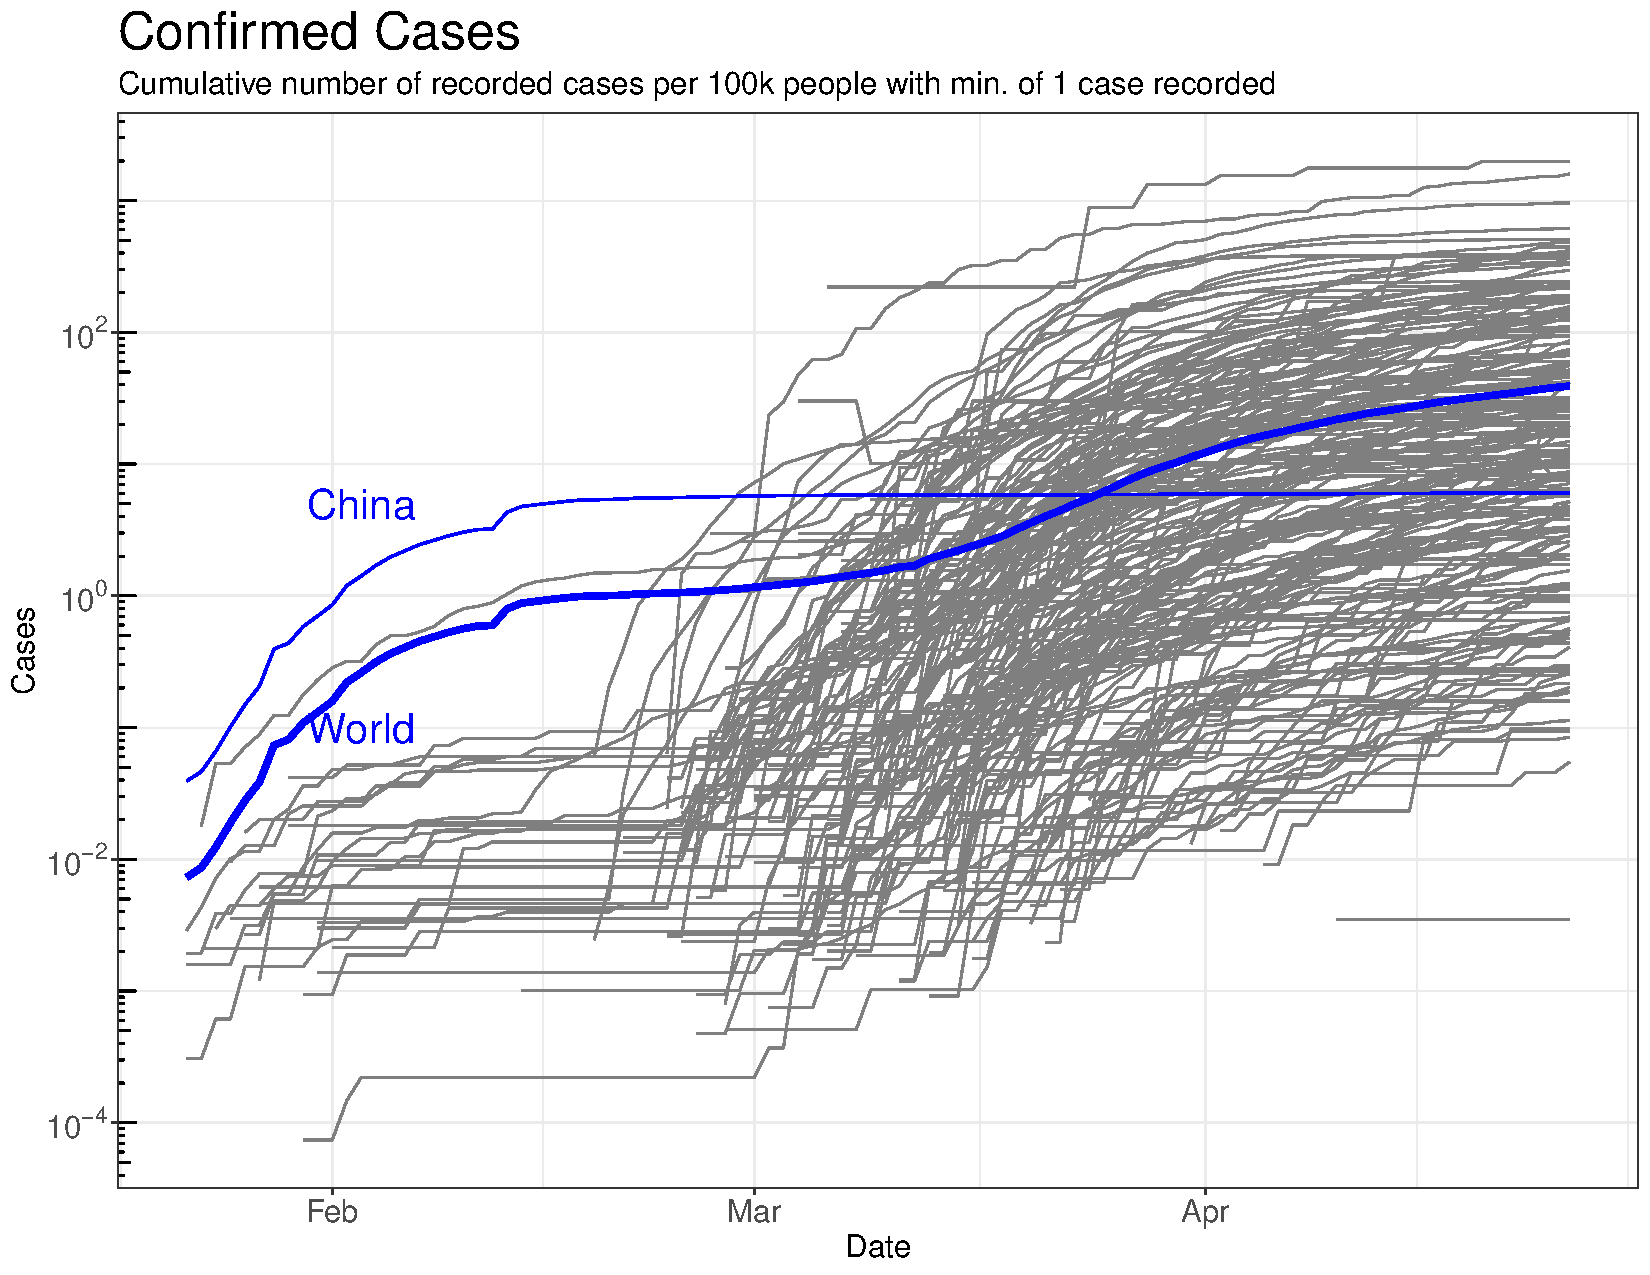
\includegraphics[width = 270pt]{Cases_cumulative_confirmed.pdf}
	\end{figure}
 \end{frame}

 \begin{frame}
 	\frametitle{COVID-19 weltweit bestätigte Todesfälle}
	\begin{figure}
		\centering
		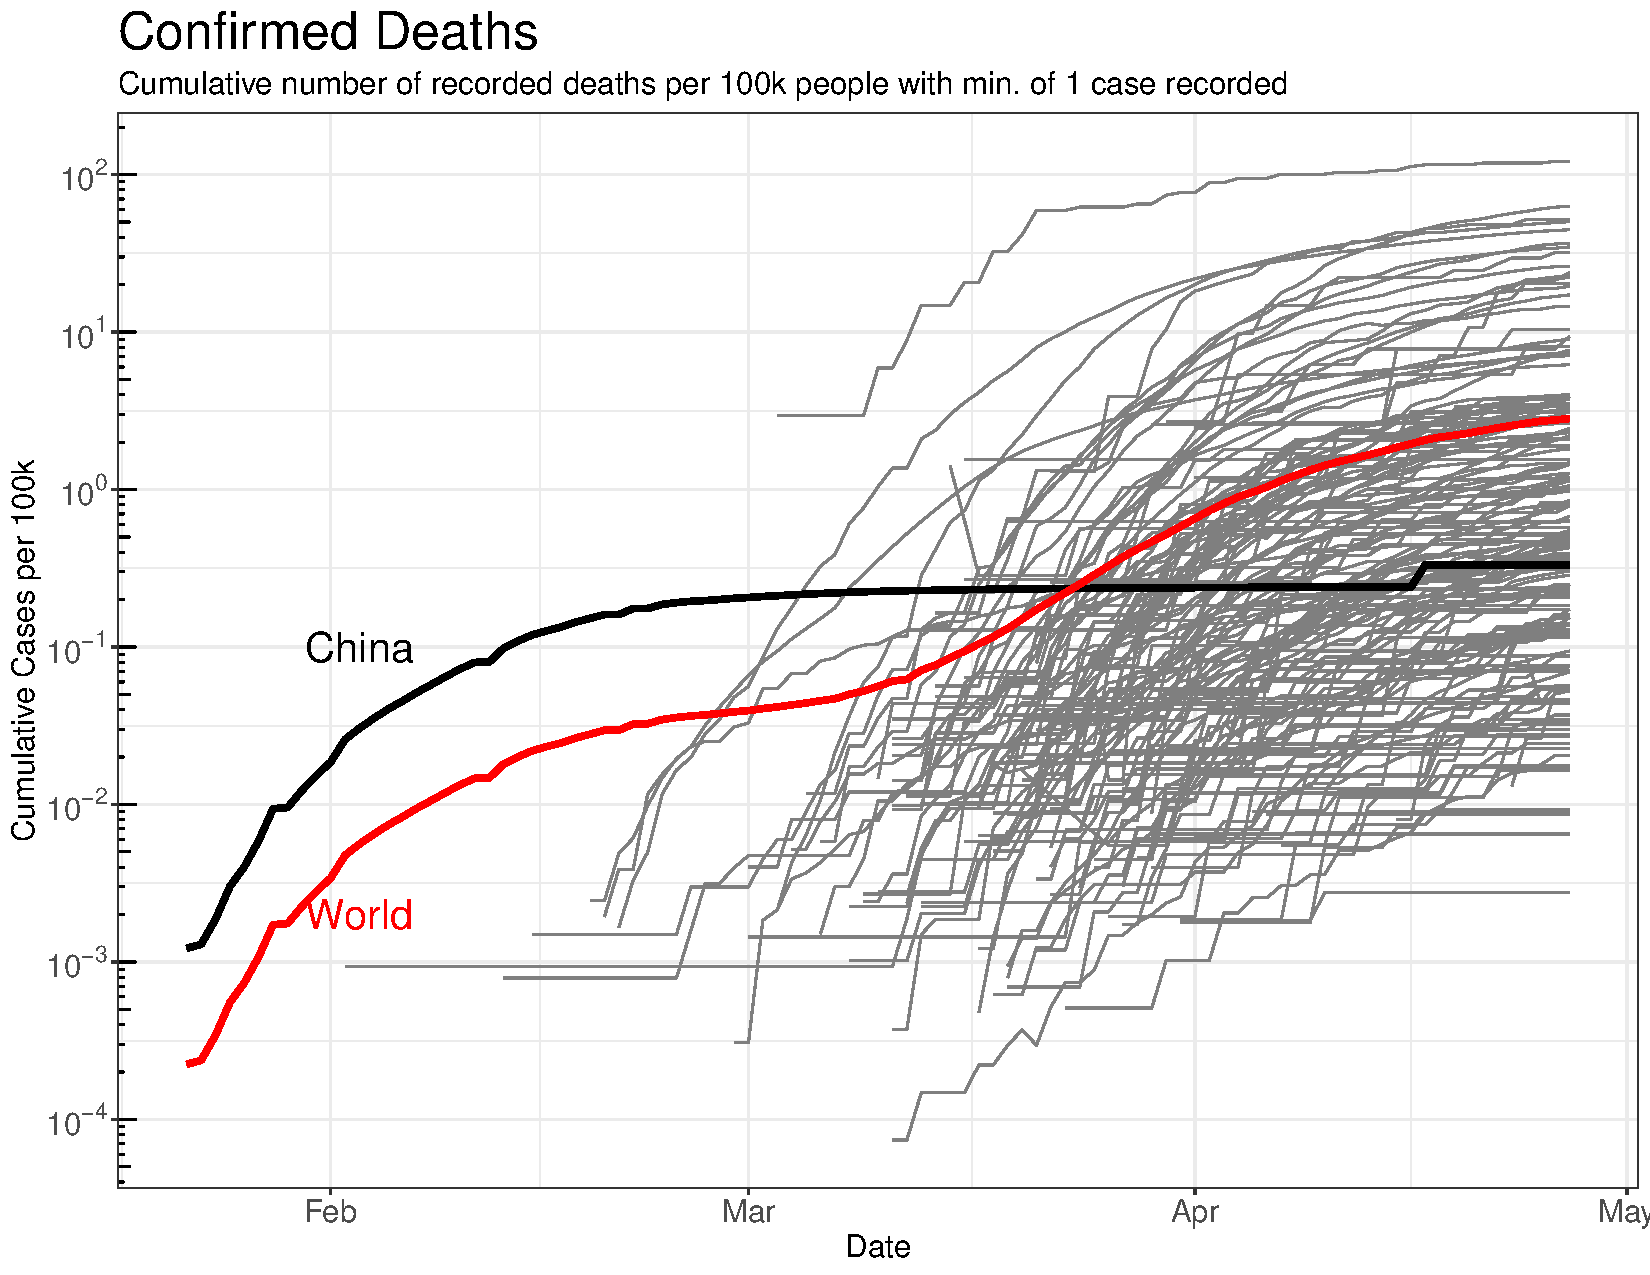
\includegraphics[width = 270pt]{Cases_cumulative_deaths.pdf}
	\end{figure}
 \end{frame}

 \begin{frame}
 	\frametitle{Zwischenergebnis}
 	\begin{itemize}
 		\item Aktuell (27. April 2020) sind weltweit etwa 40 Fälle und 3 Todesfälle pro 100k Einwohner gemeldet.
 		\item Durch logarithmische Darstellung sind zwei Infektionswellen erkennbar. Die erste Infektionswelle ist durch China dominiert.
 		\item Geografisch besonders Europa und die USA betroffen. 
 		\item Für die meisten afrikanischen Staaten sind kaum Fälle gemeldet.
 	\end{itemize}
 \end{frame}

\section{Wachstumsfaktoren der kumulativen Fälle und Todesfälle}
\begin{frame}
	\frametitle{Wiederholung: Wachstumsfaktor und geometrisches Mittel}
	\begin{boxeded}
		\textbf{Definition 1} \textit{Wachstumsfaktor}\\
		Sei $C_0, C_1, C_2, ... C_n$ eine Zeitreihe von kumulativen Fallzahlen zu den Zeitpunkten $0, 1, ..., n$. Dann ist für $i = 1, ..., n$ der i-te Wachstumsfaktor $x_i$ gegeben durch $$ x_i = \frac{C_i}{C_{i-1}}.$$
		Dadruch ergeben sich die kum. Fallzahlen zum Zeitpunkt $n$ durch $C_n = C_0 \cdot x_1 \cdot x_2 \cdot ... \cdot x_n$.
	\end{boxeded}
	\pause
	\emph{Beispiel}: Deutschland $C_{01.03.} = 130; C_{02.03.}= 159 \Rightarrow x_{02.03.}=\frac{159}{130}=1.22$
\end{frame}

\begin{frame}
	\frametitle{Wiederholung: Wachstumsfaktor und geometrisches Mittel}
	\begin{boxeded}
		\textbf{Definition 2} \textit{Geometrisches Mittel}\\
		Das geometrische Mittel zu den Wachstumsfaktoren $x_1, x_2, ..., x_n$ ist gegeben durch $$\bar{x}_{geom} = (x_1 \cdot x_2 \cdot ... \cdot x_n)^{1/n}.$$ Daraus ergibt sich $C_n = C_0 \cdot x_1 \cdot x_2 \cdot ... \cdot x_n = C_0 \cdot (\bar{x}_{geom})^n$.
	\end{boxeded}
	\pause
	Wir betrachten im Folgenden den \emph{rolling geometric mean} der vergangenen 7 Tage. Dazu berechnen wir für jeden Zeitpunkt $i$ $$\bar{x}_{i, geom} = (x_i \cdot x_{i-1} \cdot x_{i-2} \cdot ... \cdot x_{i-6})^{1/7}.$$
\end{frame}

\begin{frame}
	\frametitle{Wachstumsfaktoren: Bestätigte Fälle}
	\begin{figure}
		\centering
		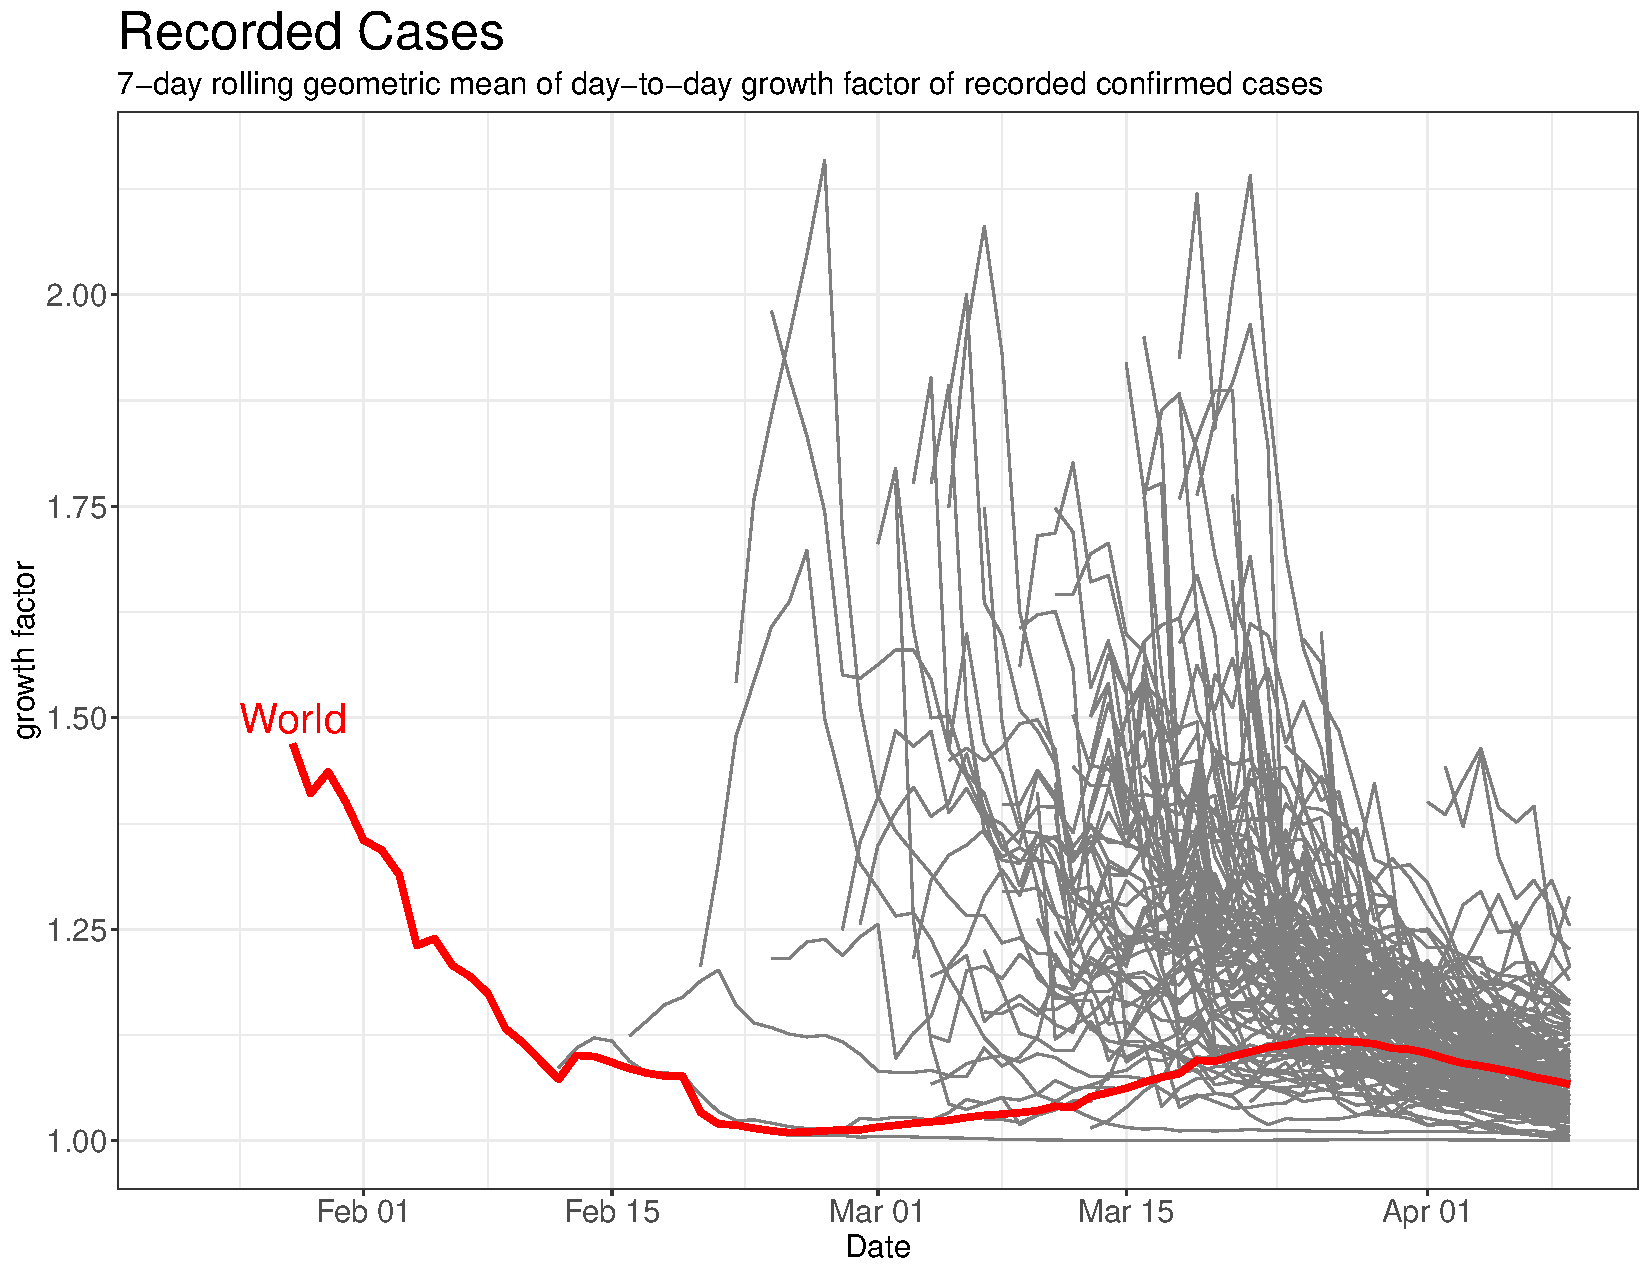
\includegraphics[width = 270pt]{GF_confirmed}
	\end{figure}
\end{frame}

\begin{frame}
	\frametitle{Wachstumsfaktoren: Todesfälle}
	\begin{figure}
		\centering
		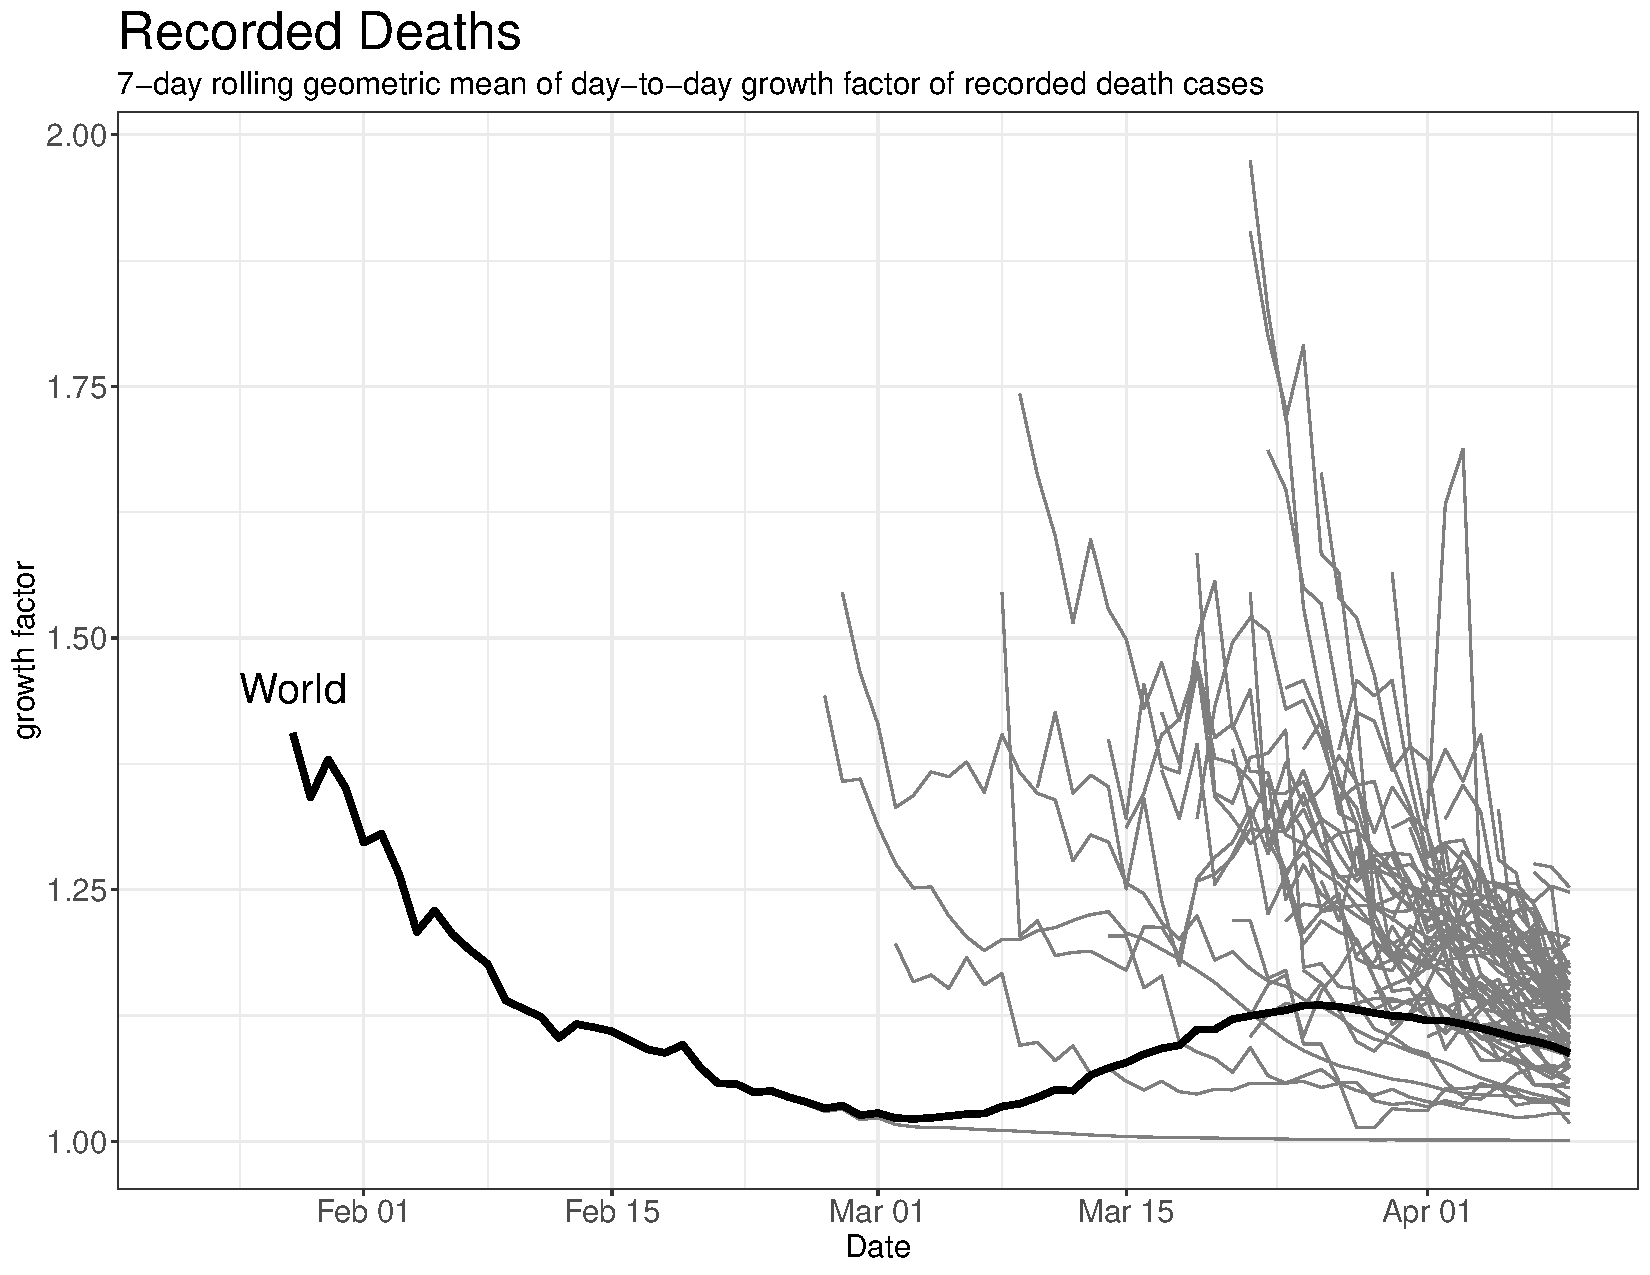
\includegraphics[width = 270pt]{GF_deaths}
	\end{figure}
\end{frame}

\begin{frame}
	\frametitle{Verdopplungszeit}
	Ausgehend von einem exponentiellen Wachstum der Form $C_n = C_0 \cdot (\bar{x}_{n, geom})^{n}$ ergibt sie die "momentane" Verdopplunszeit $dt_i$ der Fallzahlen durch $$dt_i = \frac{ln(2)}{ln(\bar{x}_{i, geom})}.$$
	\pause
	\emph{Beispiel}: Erinnerung: Wachstumsfaktor von Deutschland am 02. März 2020 $$x_{02.03.} = 1.22 \Rightarrow dt_{02.03.} = \frac{ln(2)}{ln(1.22)} = 3.49$$ 
	\pause
	Bei einem Wachstum mit Faktor 1.22 würde sich die Anzahl an Fällen also alle 3.49 Tage verdoppeln.
	
\end{frame}

\begin{frame}
	\frametitle{Verdopplungszeit: Bestätigte Fälle}
	\begin{figure}
		\centering
		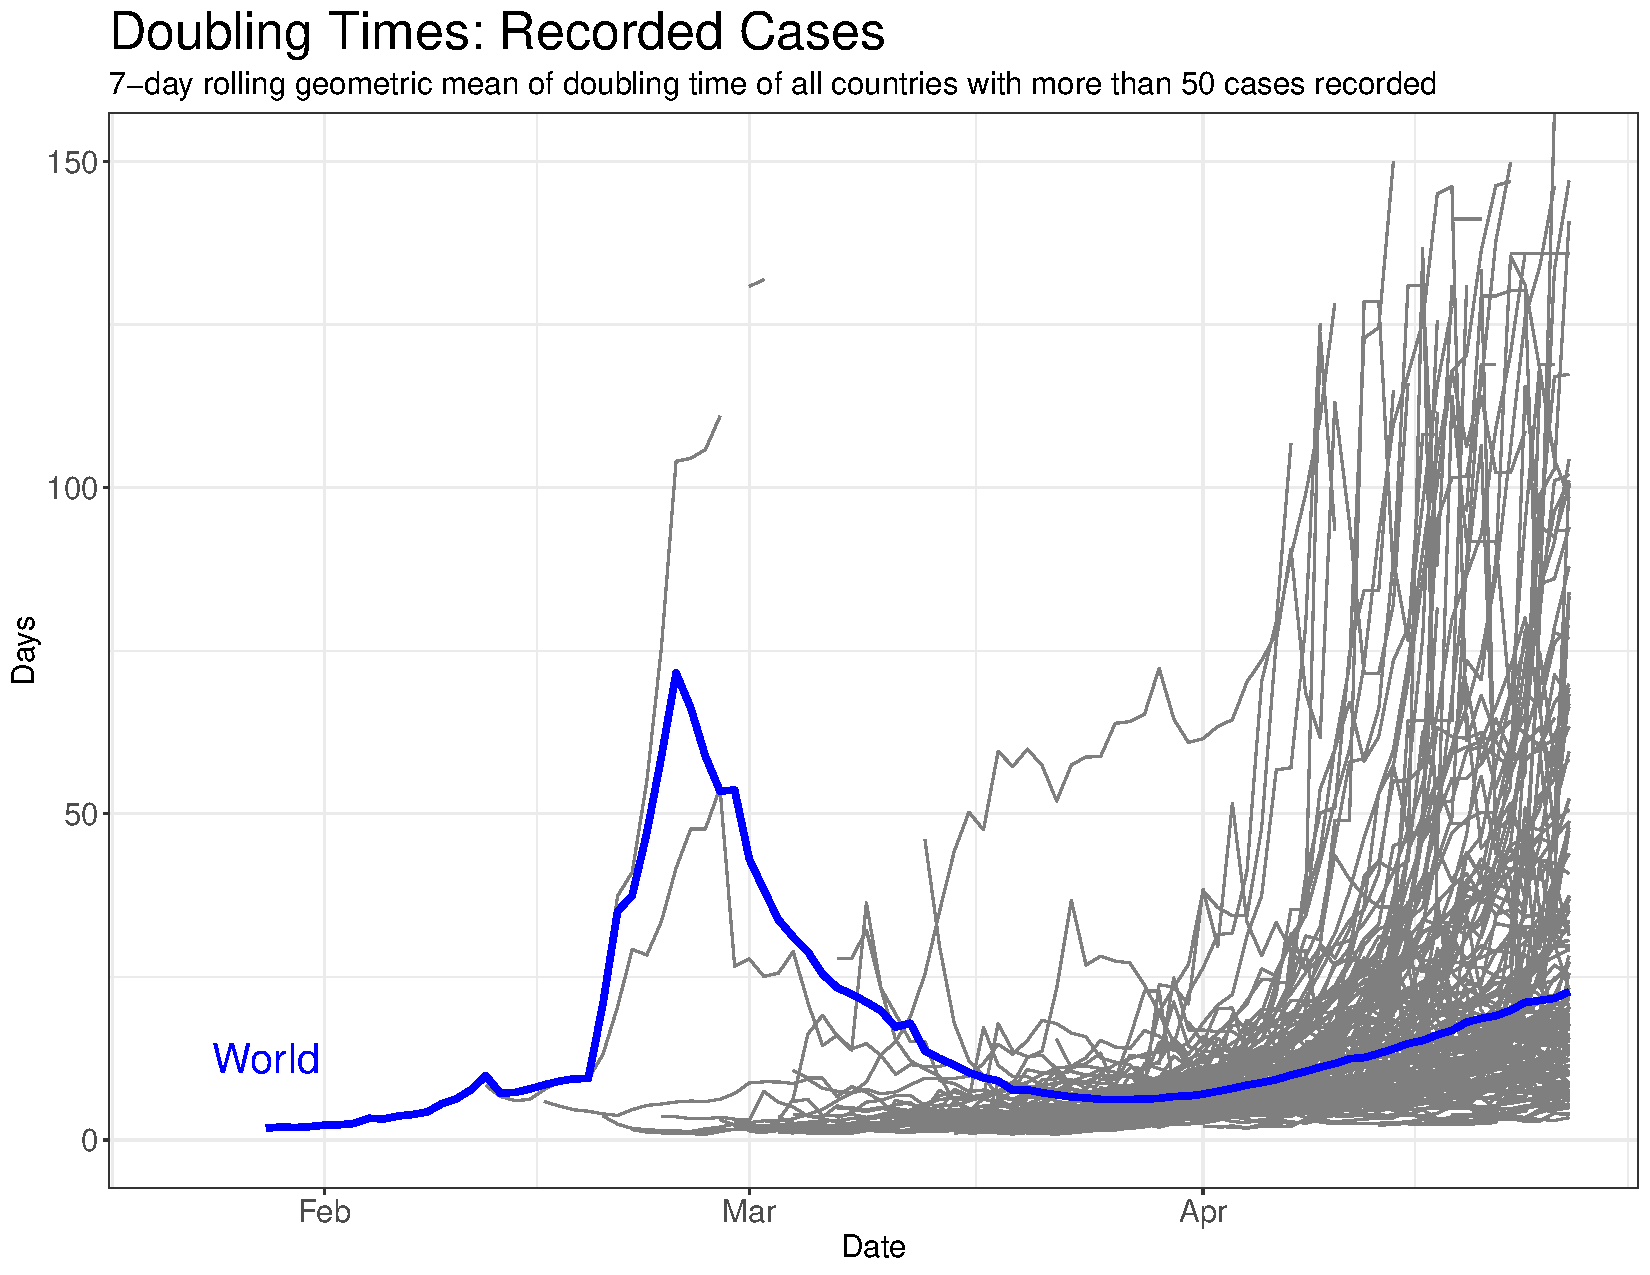
\includegraphics[width = 270pt]{DT_confirmed}
	\end{figure}
\end{frame}

\begin{frame}
	\frametitle{Verdopplungszeit: Todesfälle}
	\begin{figure}
		\centering
		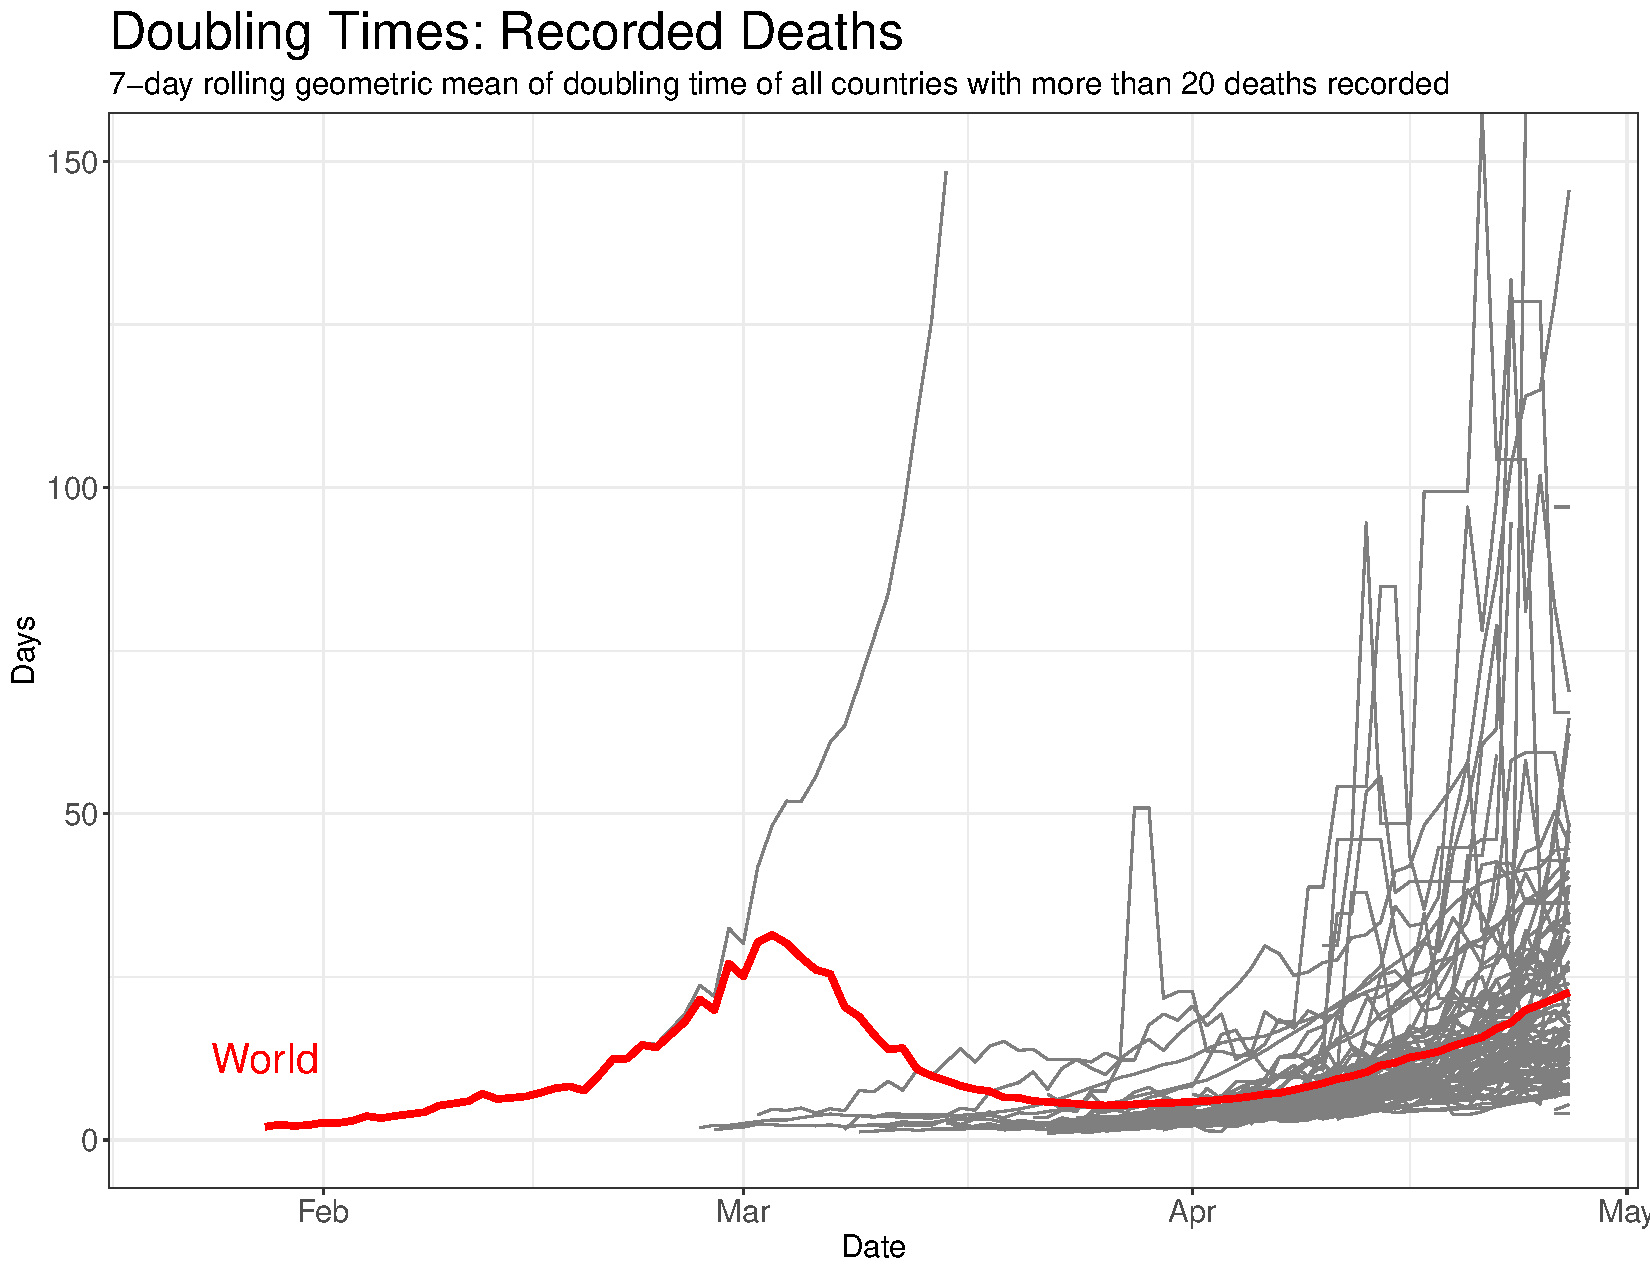
\includegraphics[width = 270pt]{DT_deaths}
	\end{figure}
\end{frame}

 \begin{frame}
 	\frametitle{Zwischenergebnis}
 	\begin{itemize}
 		\item Unter der Annahme eines exponentiellen Wachstums lassen sich kumulativen Fällen und Todesfällen über die Berechnung von Wachstumsfaktoren und Verdopplungszeiten direkt miteinander vergleichen. 
 		\item Aktuell (27. April 2020) besteht ein Wachstumsfaktor der kumulativen Fälle von etwa 1.03, was einer Verdopplungszeit von etwa 24 Tagen entspricht.
 		\item Das lokale Minimum der Wachstumsfaktoren (bzw. lokales Maximum der Verdopplungszeit) der weltweiten Fälle liegt etwa eine Woche vor dem lokalen Minimun der Wachstumsfaktoren der weltweiten Todesfälle.
 		\item Mitte-Ende März tritt sowohl bei den Wachstumsfaktoren von Fällen und Todesfällen ein lokales Maximum der Wachstumsfaktoren (bzw. lokales Minimum der Verdopplungszeit) auf.
 	\end{itemize}
 \end{frame}

\section{Diskussion}
\begin{frame}
	\frametitle{Diskussion}
	\begin{itemize}
		\item Daten geben maximal eine untere Schranke der Zahl der Fälle und Todesfälle an.
		\item Weltweit zwei Infektionswellen, wobei die Erste von China dominiert ist.
		\item Unter Annahme eines exponentiellen Wachstums zeigt sich das Maximum der zweiten Infektionswelle Mitt-Ende März.
		\item Weltweit sind die Wachstumsfaktoren in den letzen Tagen rückläufig.
	\end{itemize}
\end{frame}

\begin{frame}
	\frametitle{Ausblick: Infektionsmaßnahmen}
	\centering
	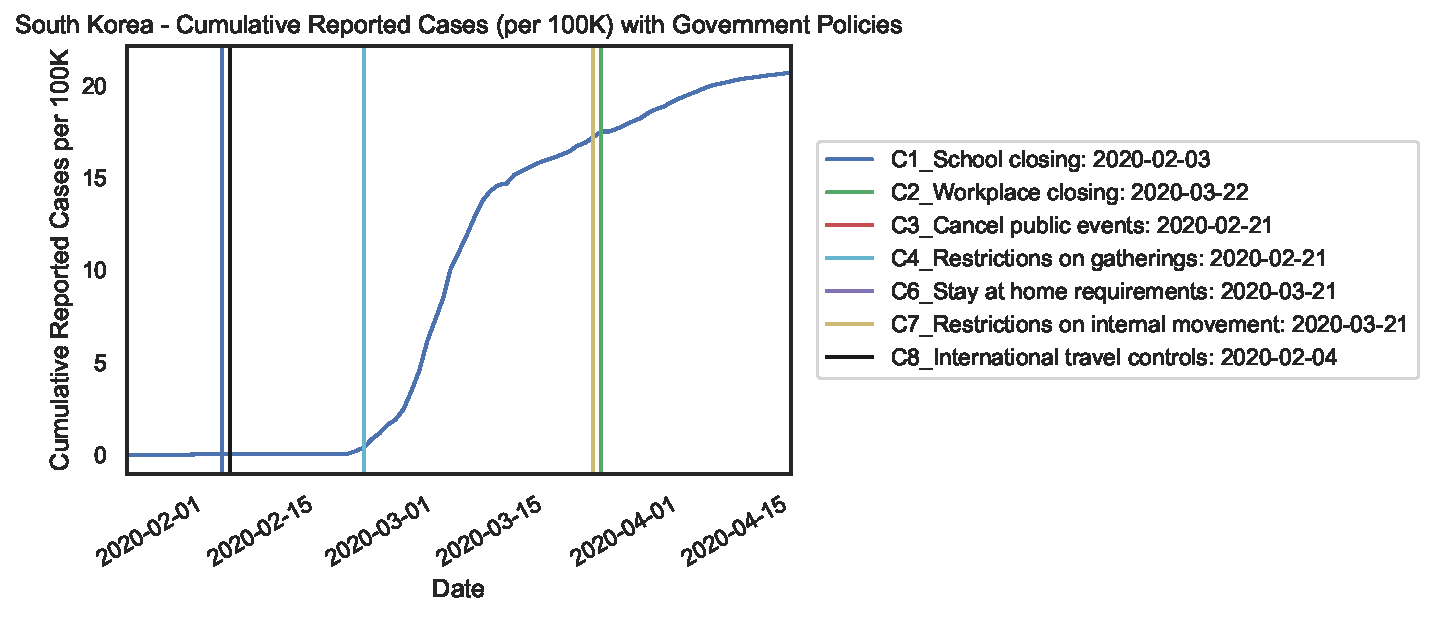
\includegraphics[width = 350pt]{korea}
\end{frame}

\begin{frame}
	\frametitle{Ende}
		\centering
		\textbf{Vielen herzlichen Dank für Ihre Aufmerksamkeit!}
\end{frame}
 
\begin{frame}
	\frametitle{Herleitung der Verdopplungszeit}
	Ausgehend von einem exponentiellen Wachstum der Form $C_n = C_0 \cdot (\bar{x}_{n, geom})^{n}$ ergibt sie die "momentane" Verdopplunszeit $dt_i$ der Fallzahlen durch $$dt_i = \frac{ln(2)}{ln(\bar{x}_{i, geom})}.$$
	\emph{Herleitung}: 
	\begin{align*} C_i \cdot (\bar{x}_{i, geom})^{dt_i} = 2 \cdot C_i 
		 &\iff (\bar{x}_{i, geom})^{dt_i} = 2 \\
	 	&\iff dt_i = \frac{ln(2)}{ln(\bar{x}_{i, geom})}.
	\end{align*}
\end{frame}

\begin{frame}
 	\frametitle{Einfluss von ``Stay at Home'' - Requirements auf die Wachstumgfaktoren}
	\begin{figure}
		\centering
		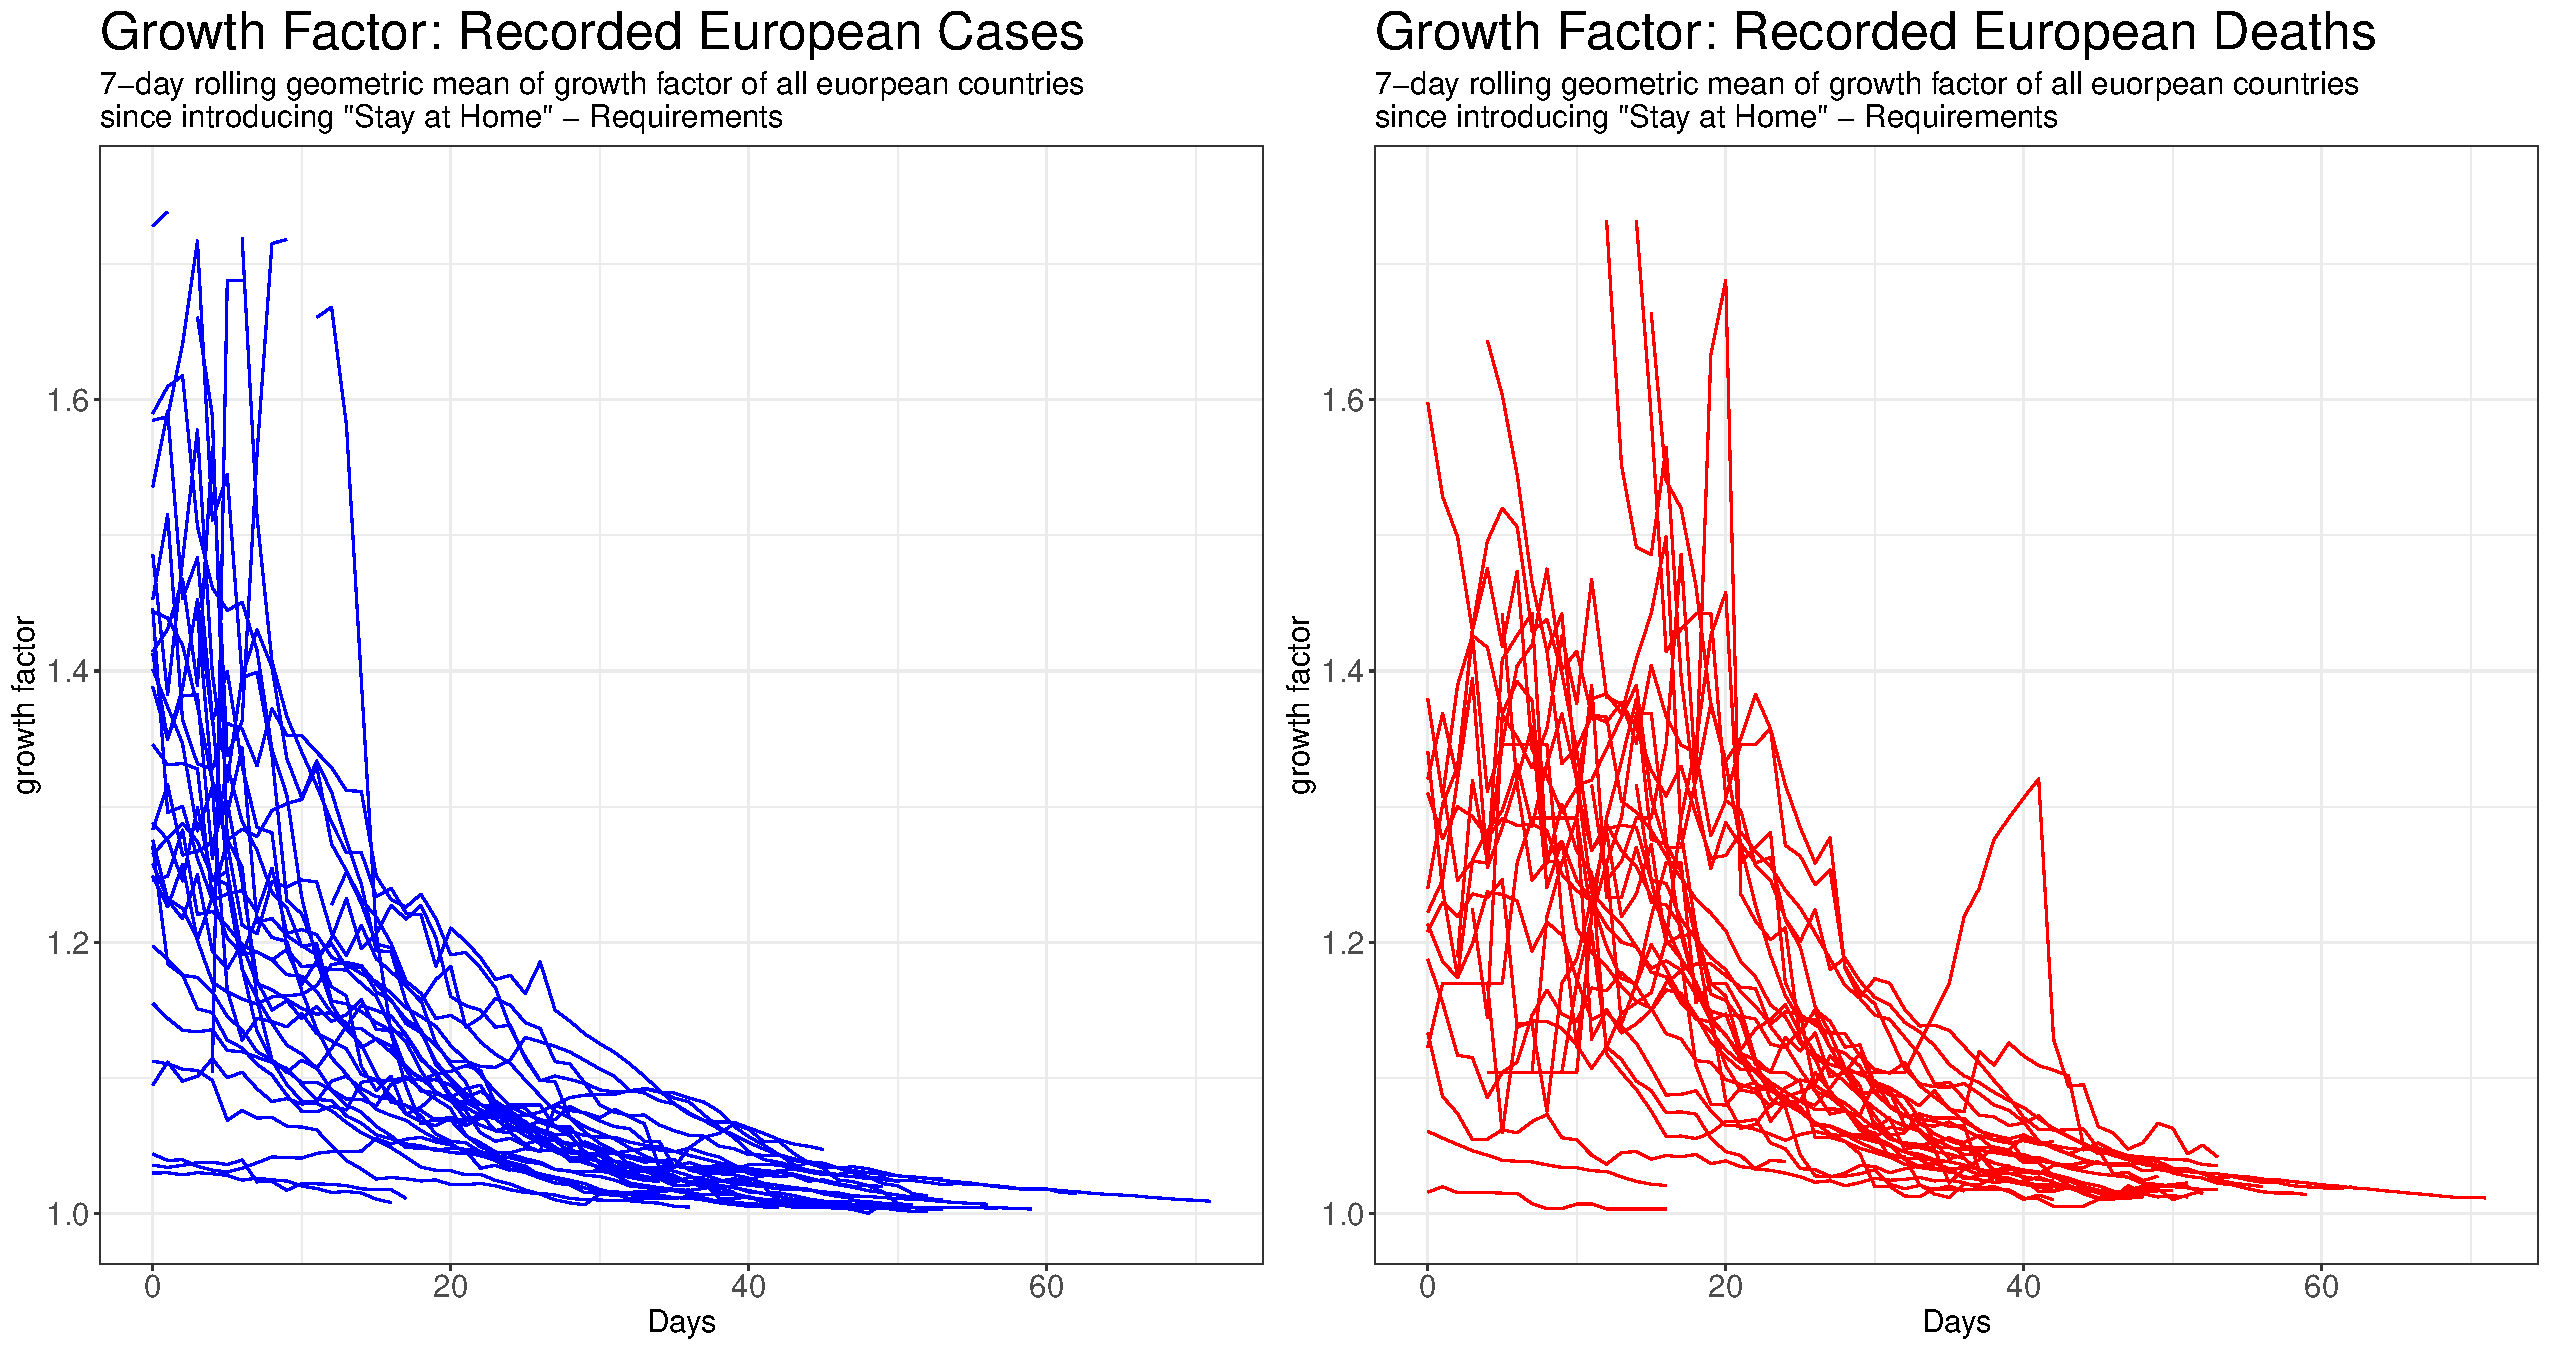
\includegraphics[width = 350pt]{plot_c6_gf.pdf}
	\end{figure}
 \end{frame}

 \begin{frame}
 	\frametitle{Einfluss von ``Stay at Home'' - Requirements auf die Verdopplungszeit}
	\begin{figure}
		\centering
		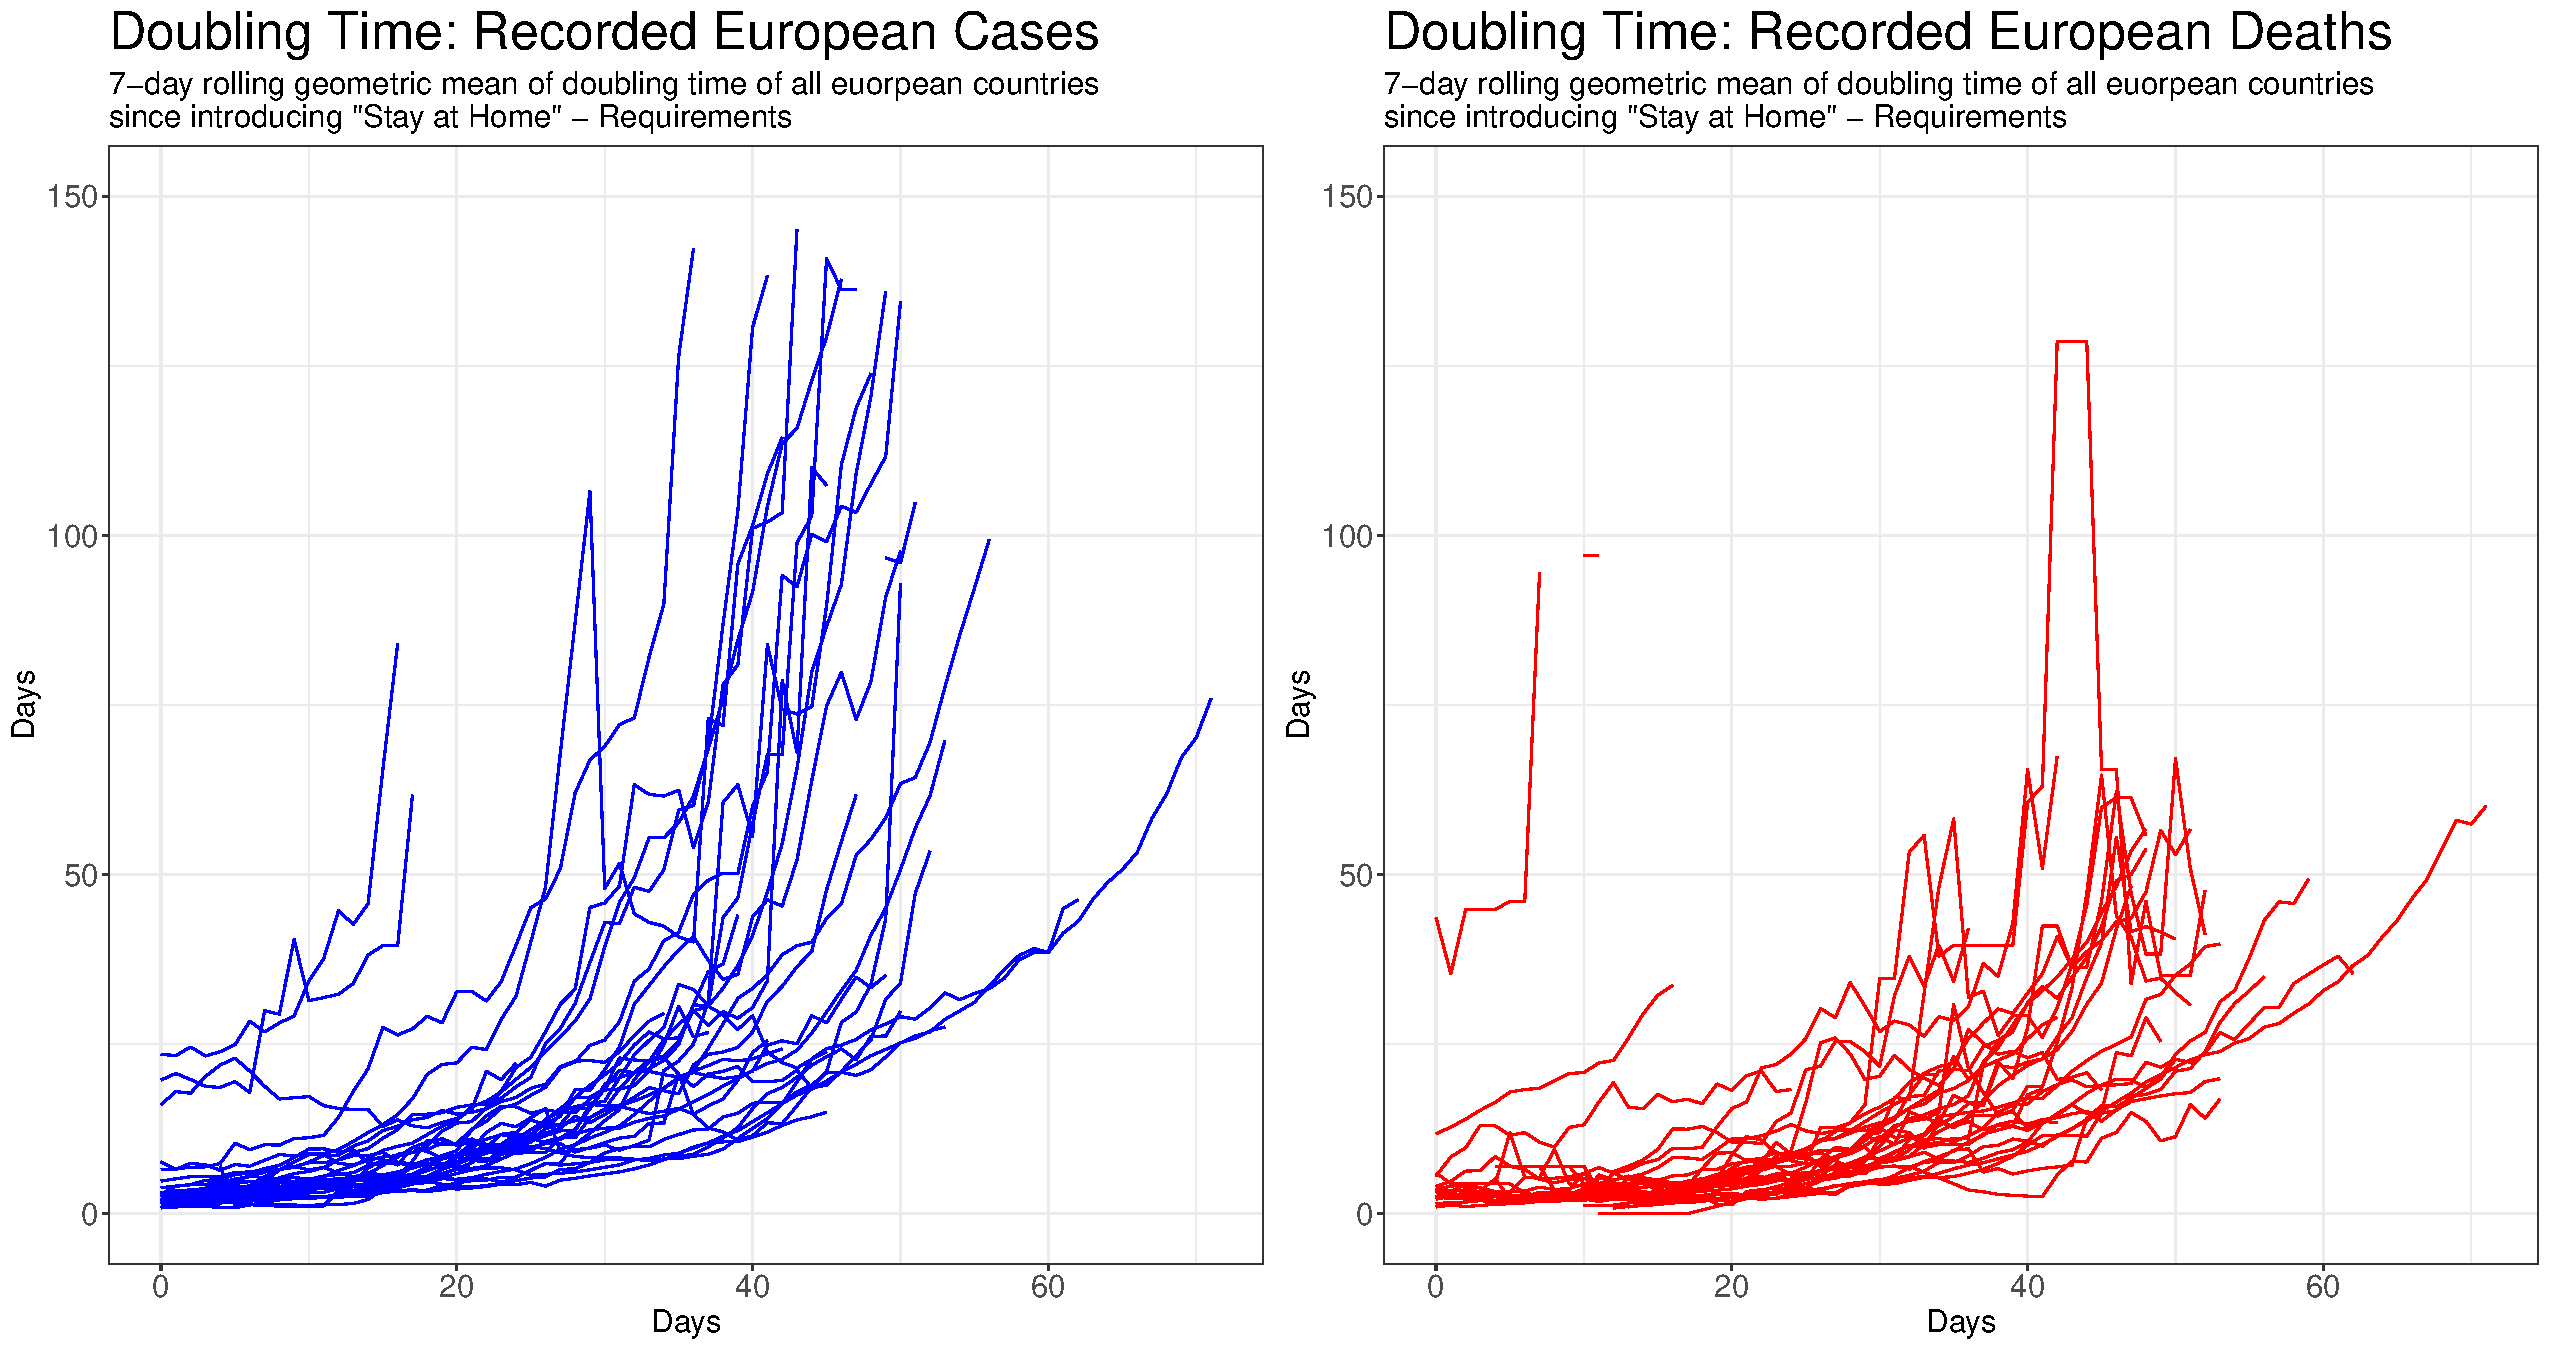
\includegraphics[width = 350pt]{plot_c6_dt.pdf}
	\end{figure}
 \end{frame}

\end{document}



\section{Einfluss von \emph{Social Distancing} auf Infektionszahlen}

\begin{frame}
	\frametitle{Infektionsmaßnahmen: Beispiel Süd Korea}
	\centering
	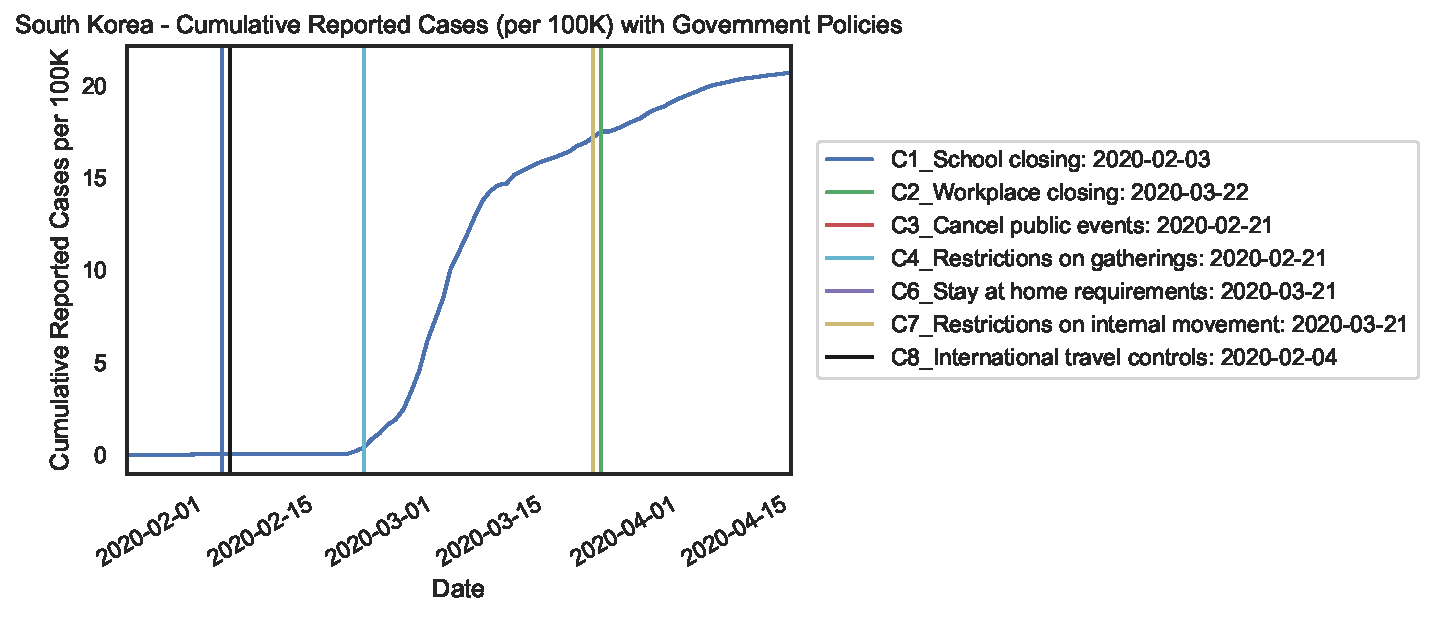
\includegraphics[width = 350pt]{korea}
\end{frame}

\begin{frame}
	\frametitle{Infektionsmaßnahmen: Einfluss von Social Distancing}
	\centering
	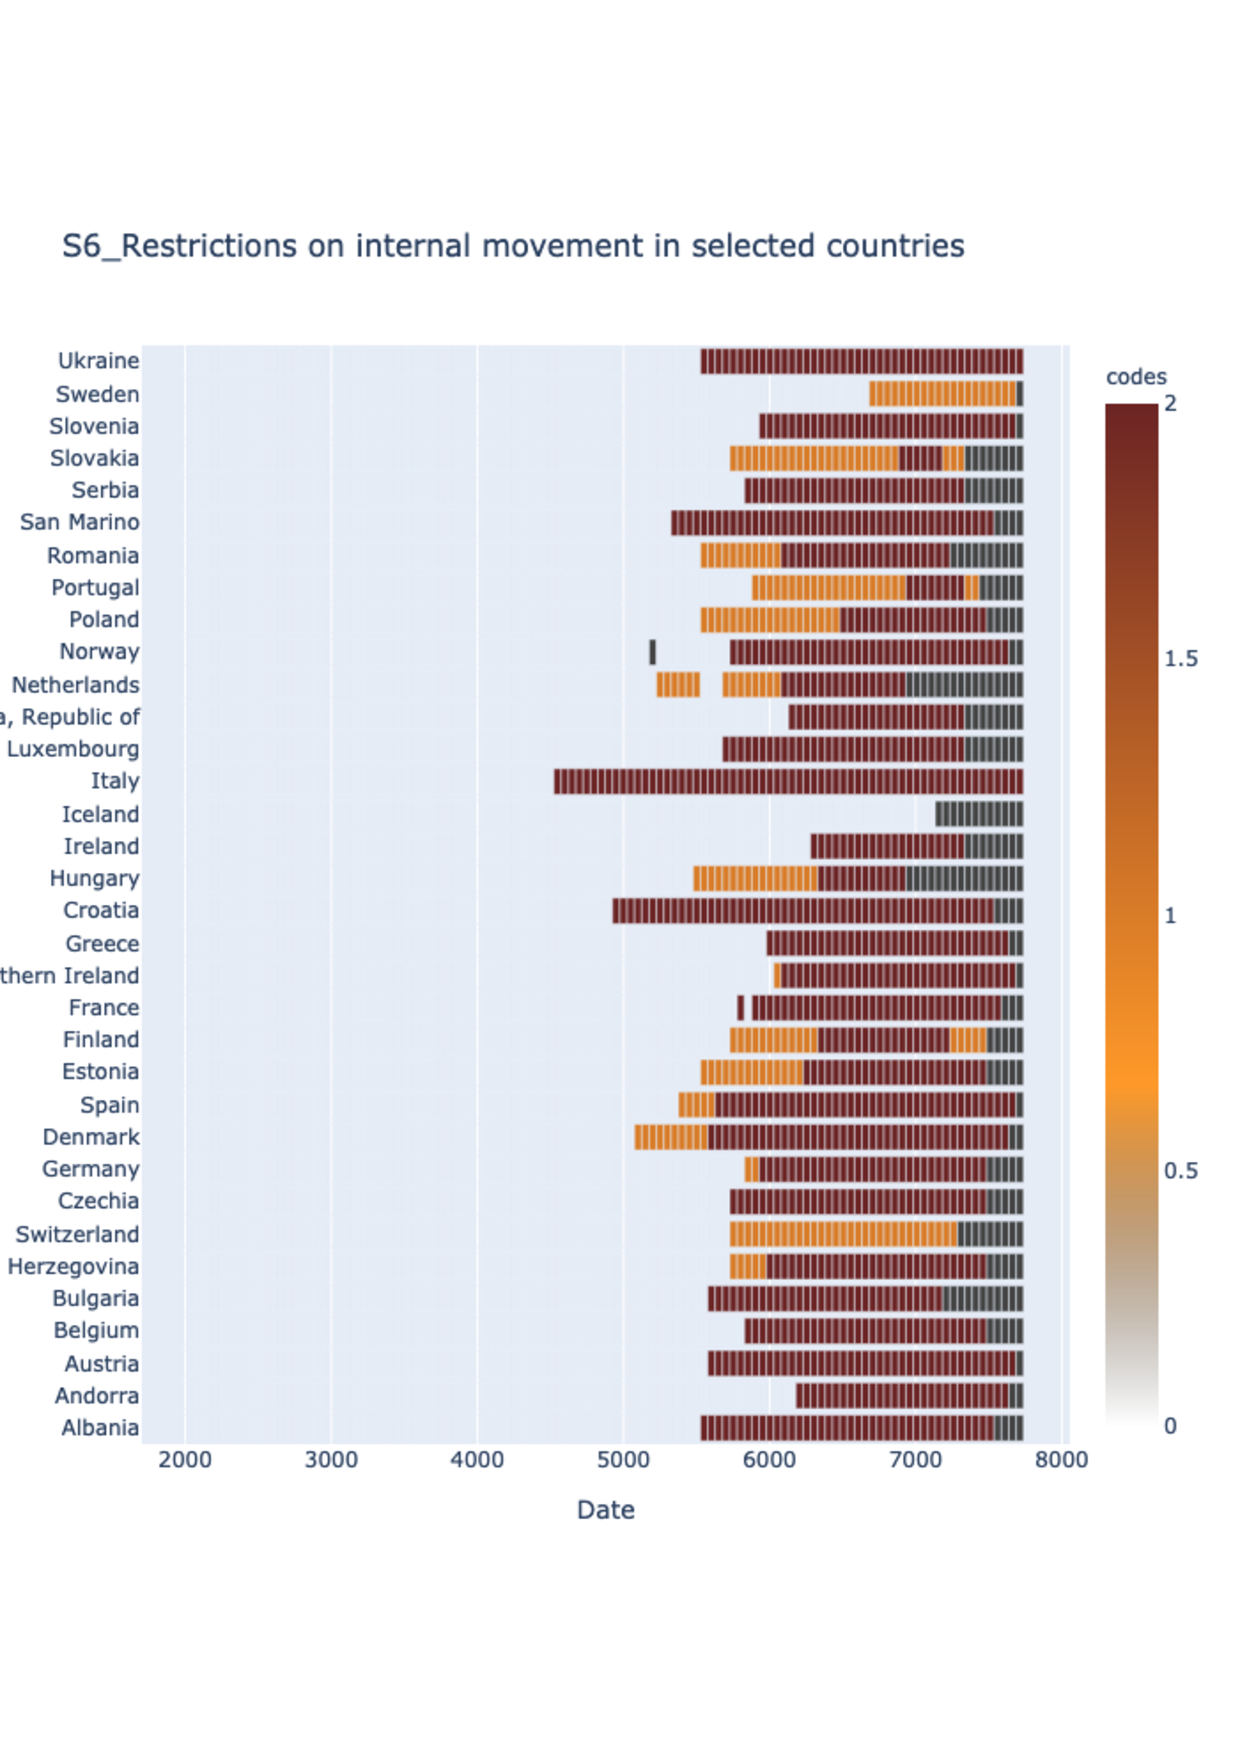
\includegraphics[width = 270pt]{responses_countries}
\end{frame}
\section{Diskussion}
\begin{frame}